

\chapter{Methodology} \label{ch:methodology}
This chapter defines the methodology used to develop the framework for testing the \gls{db}. The chapter is divided into several sections, each focusing on a specific aspect of the methodology. The first section introduces the development process as a whole, including a detailed plan with measurable milestones to ensure a systematic and robust development. The  second section discusses the first milestone which describes the test setup, including \gls{cs}, \gls{sw} algorithm, and \gls{hil} system. The third section provides an overview of the \gls{ds} used for training and testing the model, including \gls{dc}, annotation, and preprocessing techniques. Furthermore it discusses the \gls{od} algorithm and its pipeline, including the selection of a pre-trained model and the training process. Finally, the fourth section covers integration techniques, including algorithm integration with \gls{cs} and synchronization with \gls{hil} system.

\section{Introduction}

The aim of this project is to develop a closed-loop framework to validate the \gls{db} \gls{sw} using a \gls{hil} system, a \gls{cs}, and a \gls{dl}-based model that can detect the \gls{db} assets. The working principle of the system is as follows:

\begin{itemize}
    \item The \gls{hil} system controls the complete test process. It contains models of all the bike control units that communicate with the \gls{db}. Moreover, rider interactions can be simulated through CAN messages.
    \item The \gls{hil} initiates a test case by triggering a specific frame on the \gls{db} via CAN. For example, it can test whether the check engine icon appears when an engine fault message is sent.
    \item After that, the \gls{hil} sends a request to the standalone \gls{sw}, which is connected to the \gls{cs}, to capture and analyze an image. This request includes a string that defines which dashboard assets are under test.
    \item The \gls{sw} then triggers an image-capturing command to the \gls{cs} and retrieves the image for analysis.
    \item The retrieved image is analyzed using the trained \gls{dl} model, and all detected objects are compiled into a list. This list is then checked to see whether it includes the assets under test.
    \item Finally, a response is sent back to the \gls{hil}, which determines whether the test case passes or fails.
\end{itemize}

Figure \ref{proj_overview} shows a graphical overview of the connection between all project components. The communication between the \gls{hil} and the \gls{db} is handled via CAN. Communication between the \gls{hil} and the \gls{sw} occurs over HTTP using Flask, while the \gls{sw} and the \gls{cs} are connected via Ethernet. The \gls{sw} uses PyTorch to run the \gls{dl} model. PyTorch is an open-source \gls{dl} framework that provides flexible tools for building, training, and deploying \gls{cnn}s.

\begin{figure}[!htb]
    \centering
    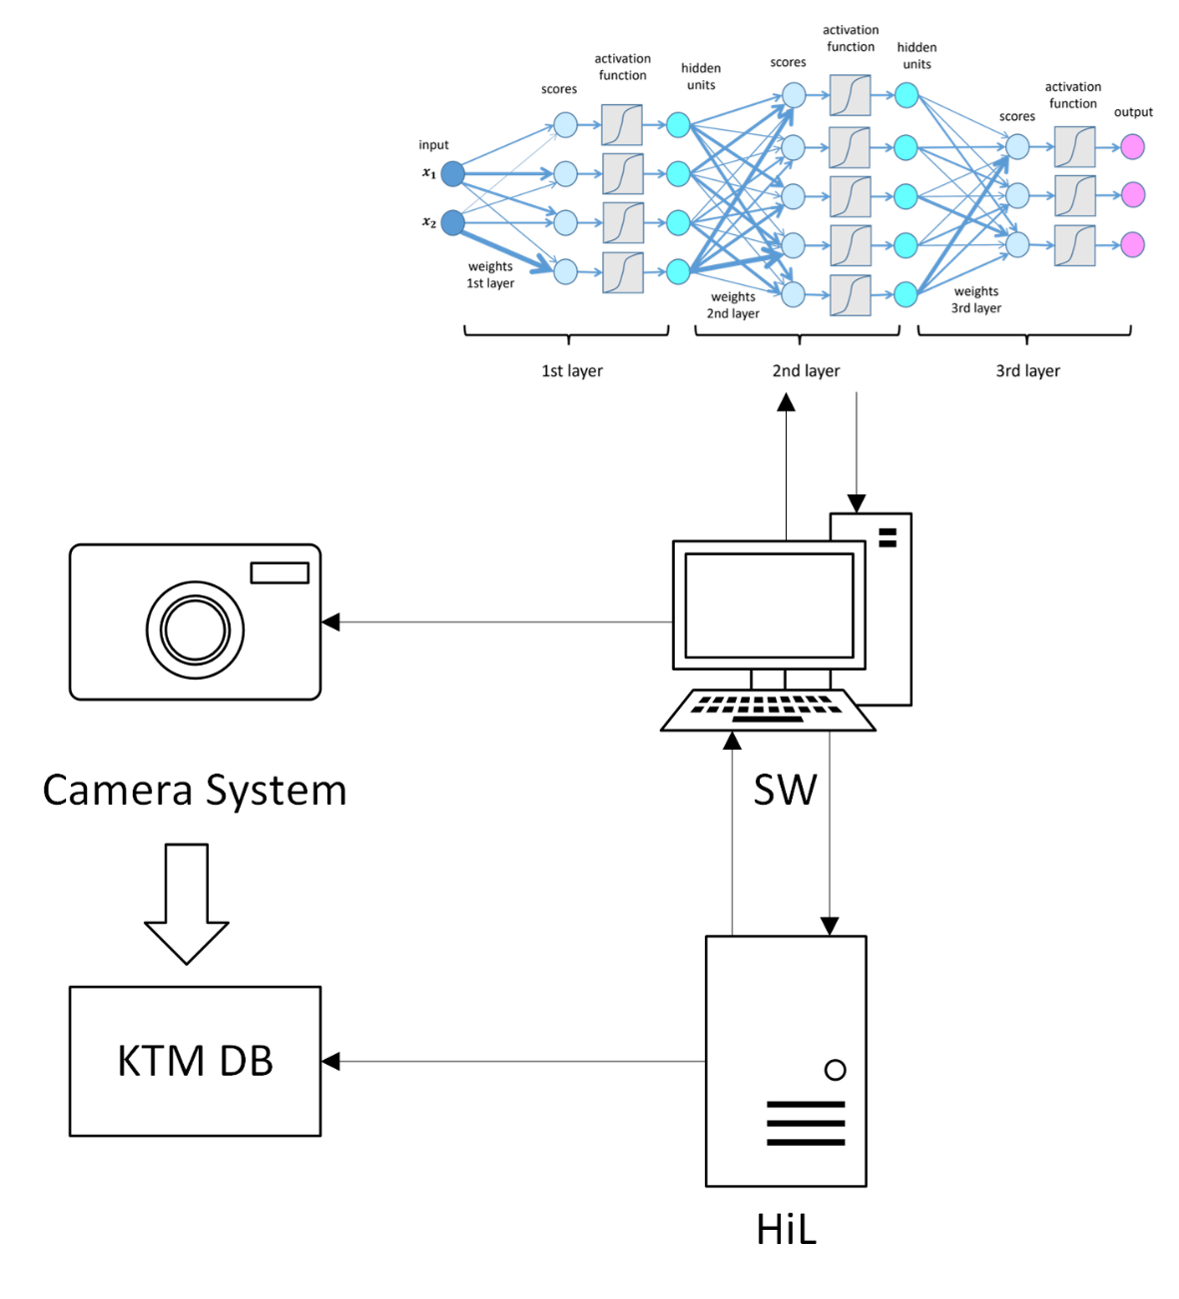
\includegraphics[width=0.6\textwidth]{Figures/Project_overview.png}
    \caption{Project overview diagram.}
    \label{proj_overview}
\end{figure}

The methodology used in this project is divided into three main milestones.  
The first milestone focuses on setting up the test environment. This includes selecting a suitable \gls{cs}, implementing light control, and integrating the \gls{hil} system. The goal is to create a fully functional closed-loop setup that can later be used to integrate the model and run detection tests.

The second milestone involves preparing a \gls{ds} in an automated way using Photoshop files. It includes image annotation, preprocessing, and augmentation to improve model generalization. Moreover, this stage includes training the selected \gls{od} model using the \gls{ds} and testing its performance on images captured from the \gls{cs}.

The third milestone is focused on integrating the trained \gls{od} model with the \gls{sw}. This \gls{sw} is responsible for synchronizing with the \gls{hil} system to carry out the complete validation cycle.


\section{Test Setup}
The test setup is an important part of the project as it provides the environment in which the \gls{db} will be tested and evaluated. The setup includes the selection of a suitable \gls{cs}, light control and the integration of a \gls{hil} system. The goal of this milestone is to develop a complete closed loop setup that is ready to integrate the model and run the detection process in the test environment. The following sections provide an overview of the test setup, including the \gls{cs}, light control and \gls{hil} integration.

\subsection{Camera System}
To evaluate the \gls{db}, the test setup relies on the \gls{cs} to capture clear and accurate images. It should be able to capture high-resolution images with a wide \gls{fov} to ensure that all relevant dashboard elements are clearly visible in each frame. Since a dedicated light control system is used to ensure consistent lighting conditions, the camera does not need to be highly sensitive to light variations. This light control approach will be explained in more detail later in this chapter. Moreover, as the \gls{db} remains stationary during testing, motion blur sensitivity is not a critical requirement.

Since a \gls{cs} was already available at KTM, it was recommended to use the existing system for this project. The chosen \gls{cs} is a high-resolution camera provided by Cognex, a company specializing in industrial-grade camera systems. This camera can capture images at a resolution of up to 12 megapixels (4096 × 3000), which is sufficient for the object detection (\gls{od}) model to accurately detect and classify dashboard elements \cite{Cognex_Camera}. Figure \ref{Cognex_Camera} shows the \gls{cs} used in the test setup.

\begin{figure}[!htb]
    \centering
    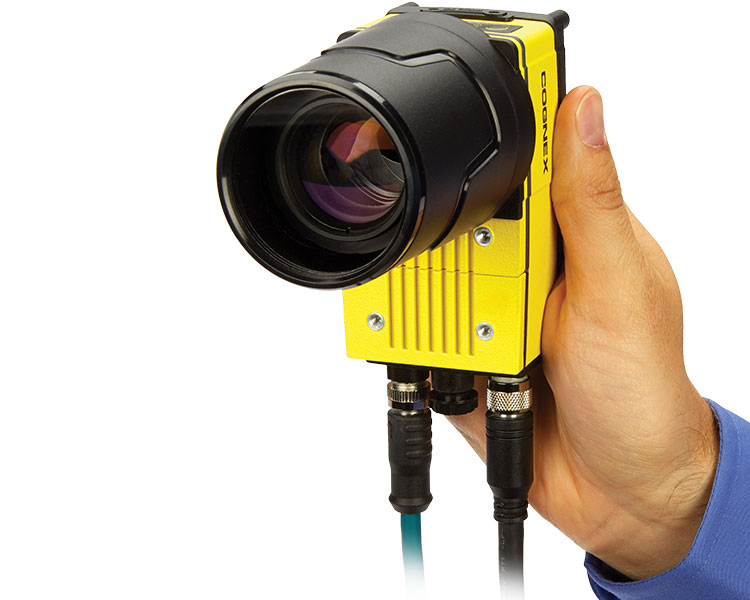
\includegraphics[width=0.5\textwidth]{Figures/In-Sight 9000 in hand.jpg}
    \caption{Cognex \gls{cs} used in the test setup \cite{Cognex_Camera}.}
    \label{Cognex_Camera}
\end{figure}

Additionally, Cognex \gls{cs} is able to communicate with external devices over Ethernet networks or serial port connections using various protocols. This allows smooth integration with the \gls{sw}, enabling reliable image capture and retrieval using \gls{telnet} and \gls{ftp} protocols through the native mode communication. The Cognex native mode communication protocol is an ASCII-based command system used to remotely control Cognex sensors. It supports communication through custom PC applications, remote serial hosts, or \gls{telnet} over Ethernet. The protocol includes two types of commands: basic (short, two-character commands) and extended (with additional functionality). When a command is sent, the sensor processes it and replies with an ASCII response. Set commands return 1 for success, 0 for unrecognized commands, or a negative number for failure, while get commands return specific values based on the request \cite{Cognex_Com}. In this project the basic comands are sufficient since it is only required to trigger an image and retrieve it. 

Set Event command was chosen to trigger an image cpaturing event, it triggers a specified event through a basic native mode command. A python code was created to trigger an image capturing using this command via \gls{telnet} and then retrieve it using \gls{ftp}, the flow chart of the code is in figure \ref{Image_capture_code}. The set Event command is SE8 baccording to Cognex documentation \cite{Cognex_Com}.

\begin{figure}[!htb]
    \centering
    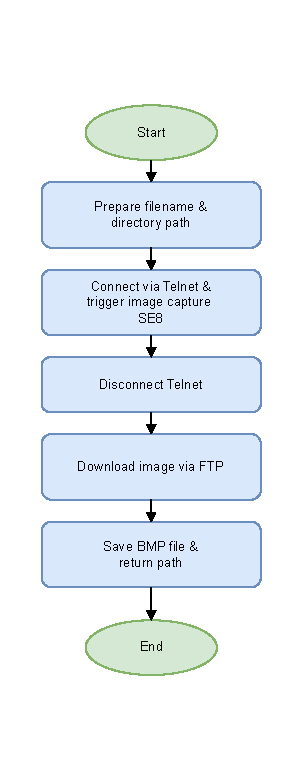
\includegraphics[width=0.3\textwidth]{Figures/diagrams/Image_Capturing.pdf}
    \caption{Process overview of image acquisition from a Cognex sensor using \gls{telnet} triggered capture and \gls{ftp} file retrieval.}
    \label{Image_capture_code}
\end{figure}

Error handling and fallback scenarios were concidered when designing the function for further integration in the complete architecture. Later in this chapter this function will be used as a first step when the \gls{hil} requests an image analysis from the standalone \gls{sw}.







\subsection{Light Control}
To ensures that the \gls{cs} captures images under a controlled optimum lighting conditions, a light control system is an essential part of the test setup. This is important for the performance of the \gls{od} model, as variations in lighting can significantly affect the quality of the detection model. The light control system should prevent any external light sources from interfering with the captured images, this is important to ensure that no glare or reflections are present in the images, which can lead to false detections or misclassifications.

KTM uses a light control system that consists of a box with aluminum frame and black walls to prevent any external light or light reflections. The box is equipped with a set of LED lights that can be adjusted to provide the desired level of illumination. The lights are positioned to ensure that the entire \gls{fov} of the camera is evenly illuminated, and they can be controlled remotely to adjust the brightness and color temperature as needed. This allows for complete control over the lighting conditions during the testing process, ensuring that the images captured by the camera are of high quality and suitable for the \gls{od} model. Figure \ref{LightControl} shows the light control system used in the test setup.

\begin{figure}[!htb]
    \centering
    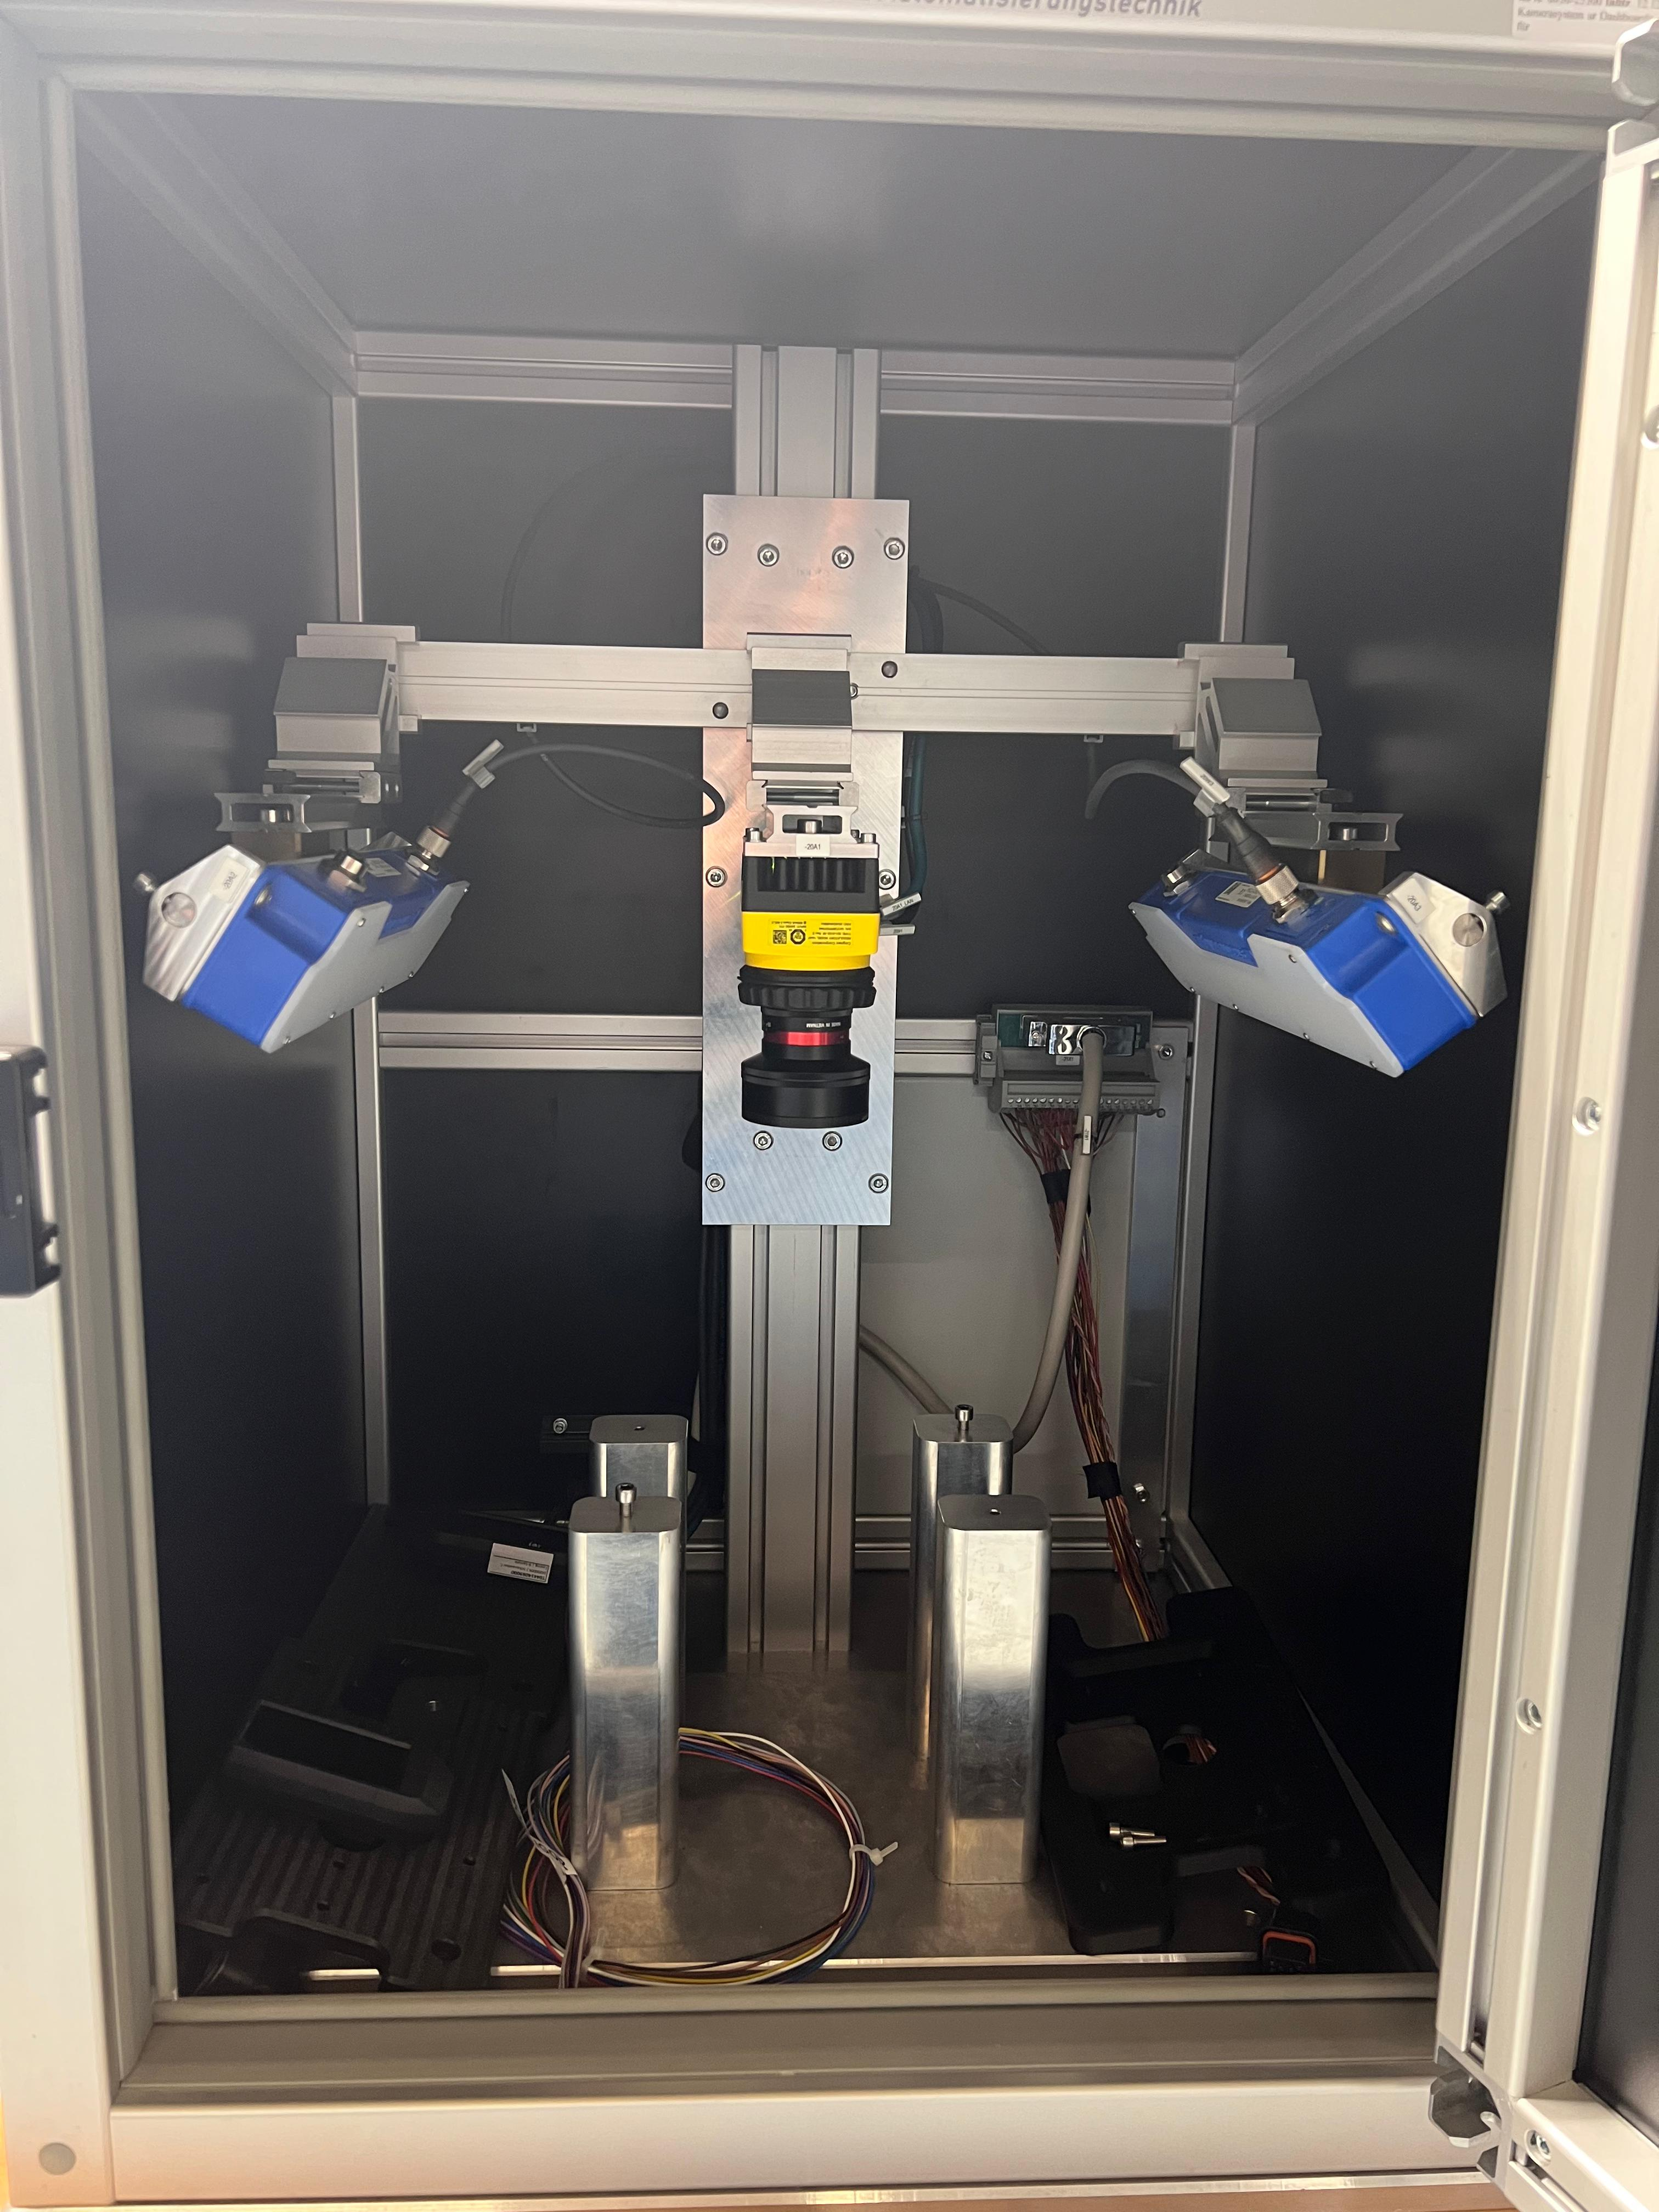
\includegraphics[width=0.6\textwidth]{Figures/Light_Control_Box.jpg}
    \caption{Light control system used in the test setup.}
    \label{LightControl}
\end{figure}

The box provides a mounting structure for the \gls{cs} to ensure that the \gls{cs} is positioned correctly and securely during the testing process. The mounting structure allows easy adjustment of the camera position and angle to ensure that the entire \gls{db} is captured in the images. Figure \ref{Camera_Mounting} shows the \gls{cs} mounted inside the light control box. The light control box also includes a mounting structure for the the \gls{db} to ensure that the distance between the \gls{cs} and the \gls{db} is consistent. Figure \ref{db_Mounting} shows the \gls{db} mounted in a secure way in the light control box. Additionally, a cable inlet is provided to allow for the connection of the \gls{cs} and the \gls{db} without compromising the light control system.

\begin{figure}[!htb]
    \centering
    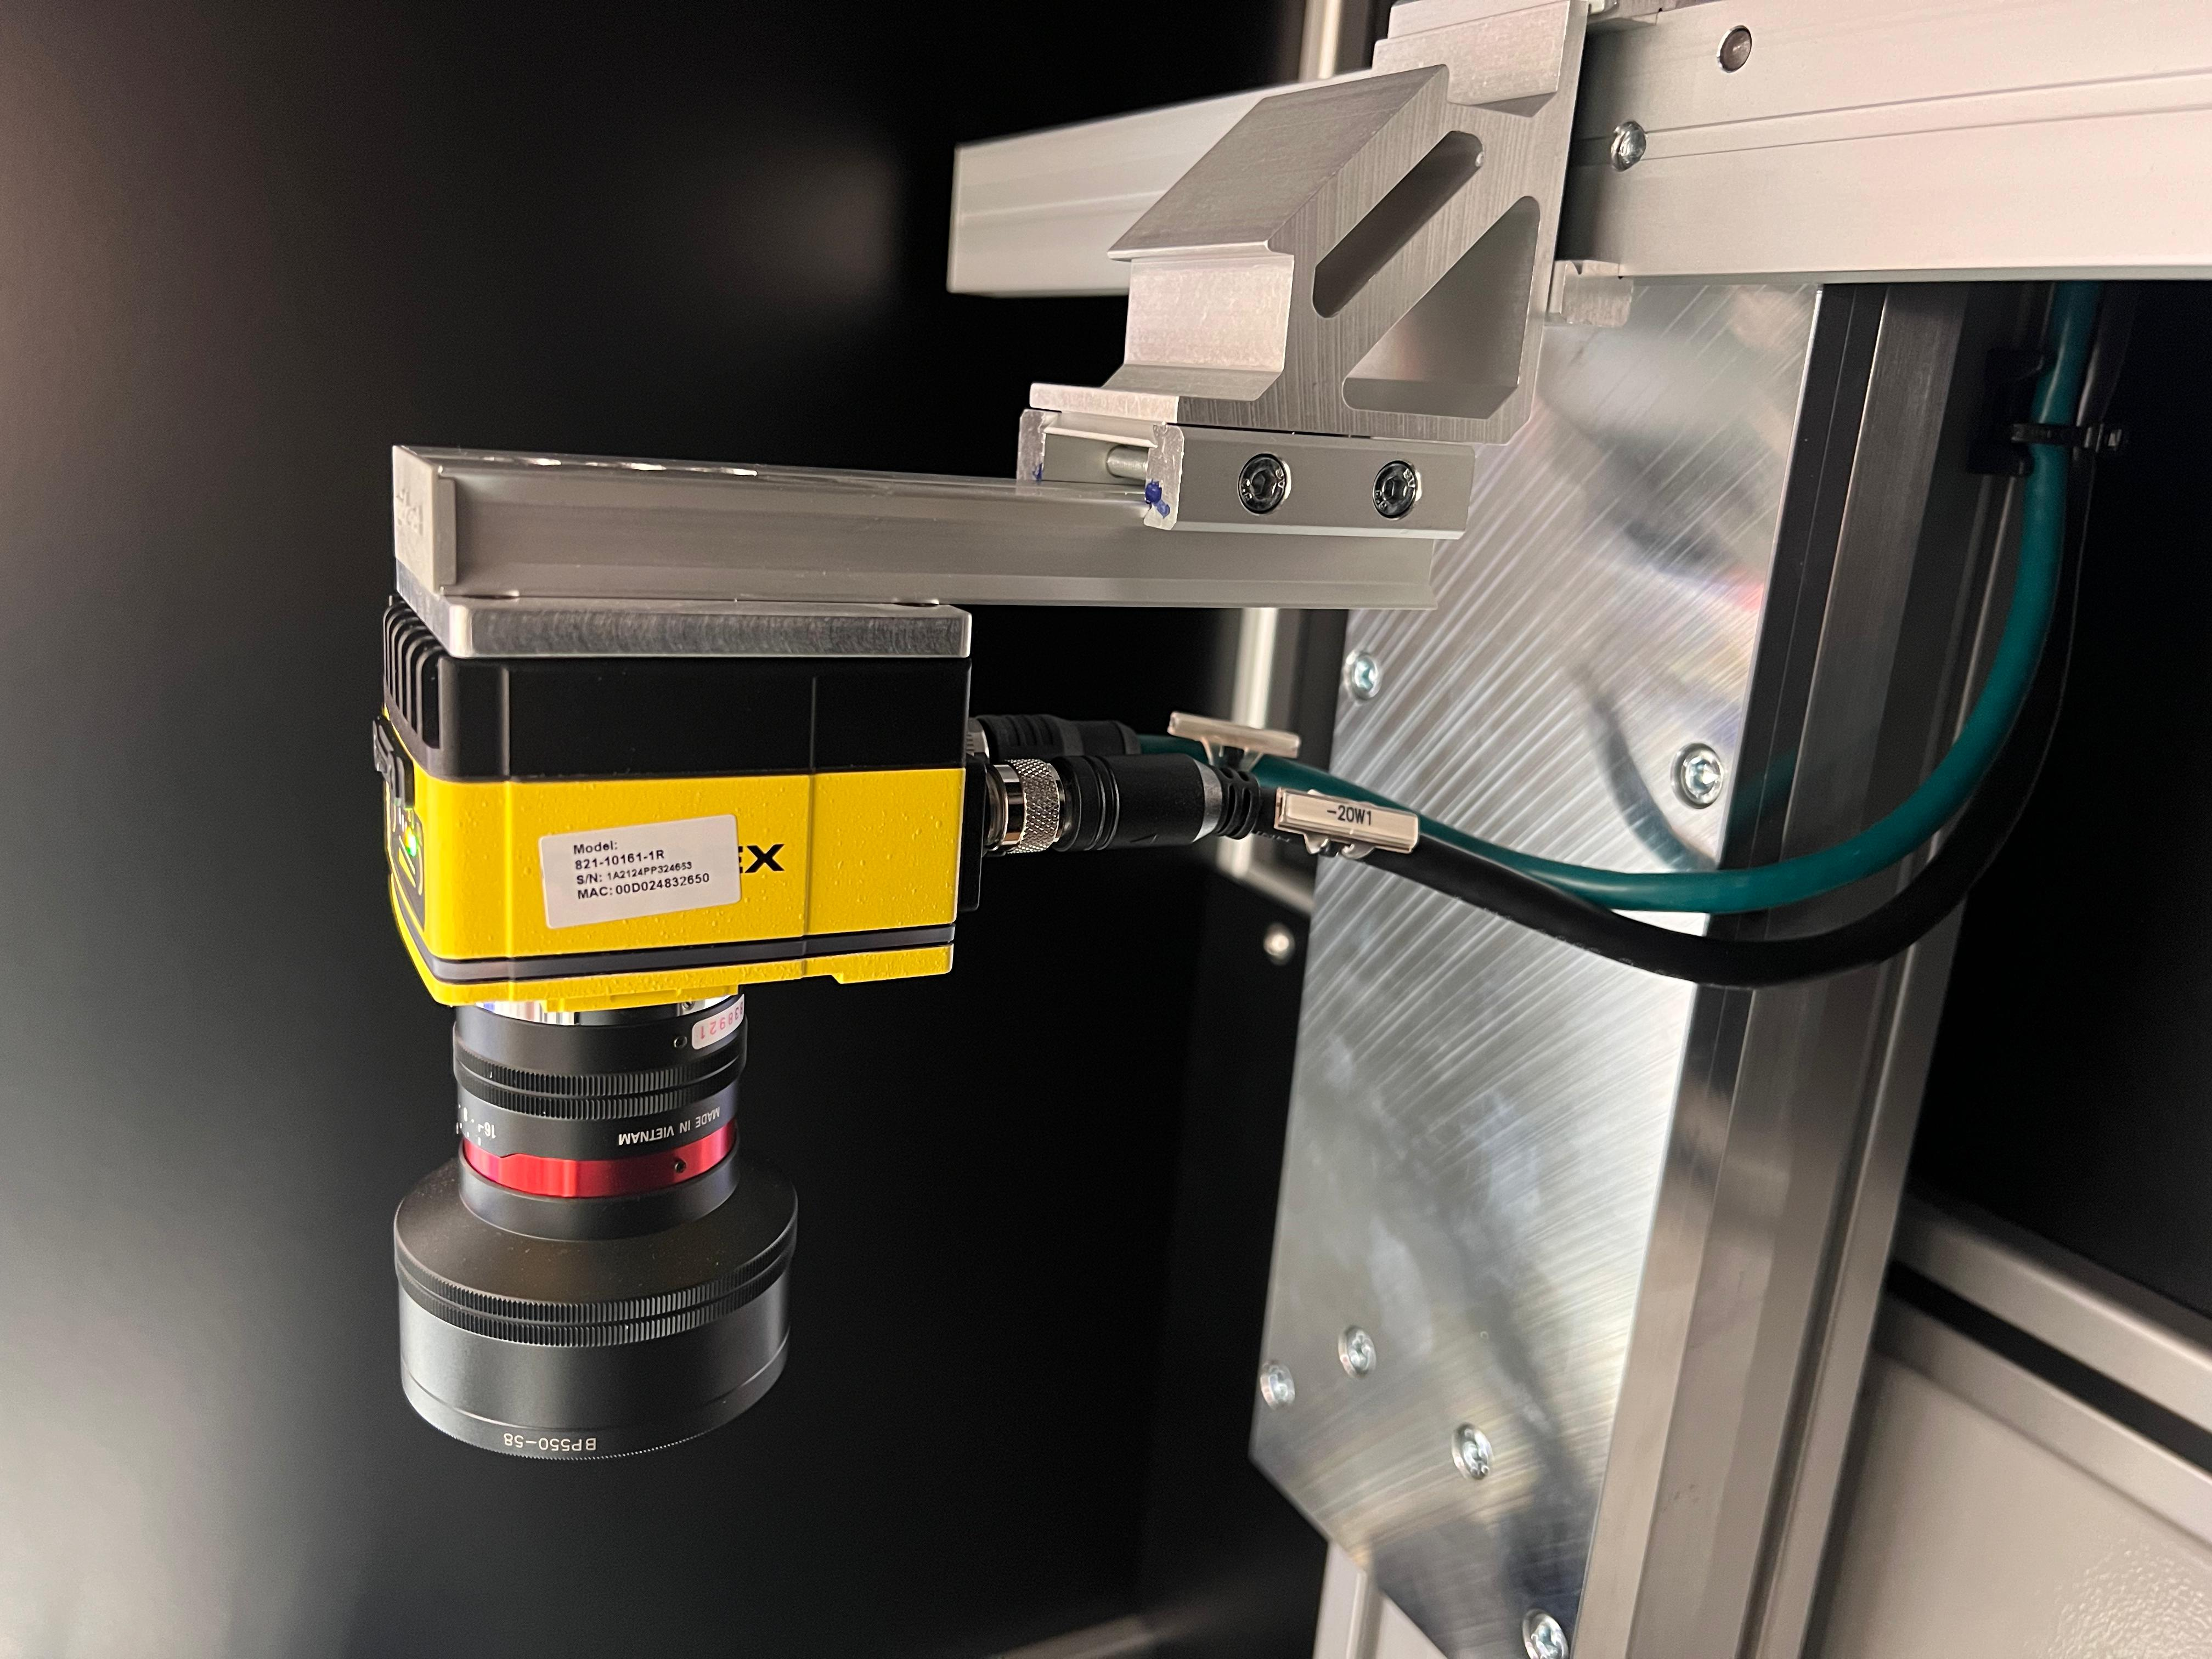
\includegraphics[width=0.6\textwidth]{Figures/Camera_Mounting.jpg}
    \caption{\gls{cs} mounted inside the light control box.}
    \label{Camera_Mounting}
\end{figure}

\begin{figure}[!htb]
    \centering
    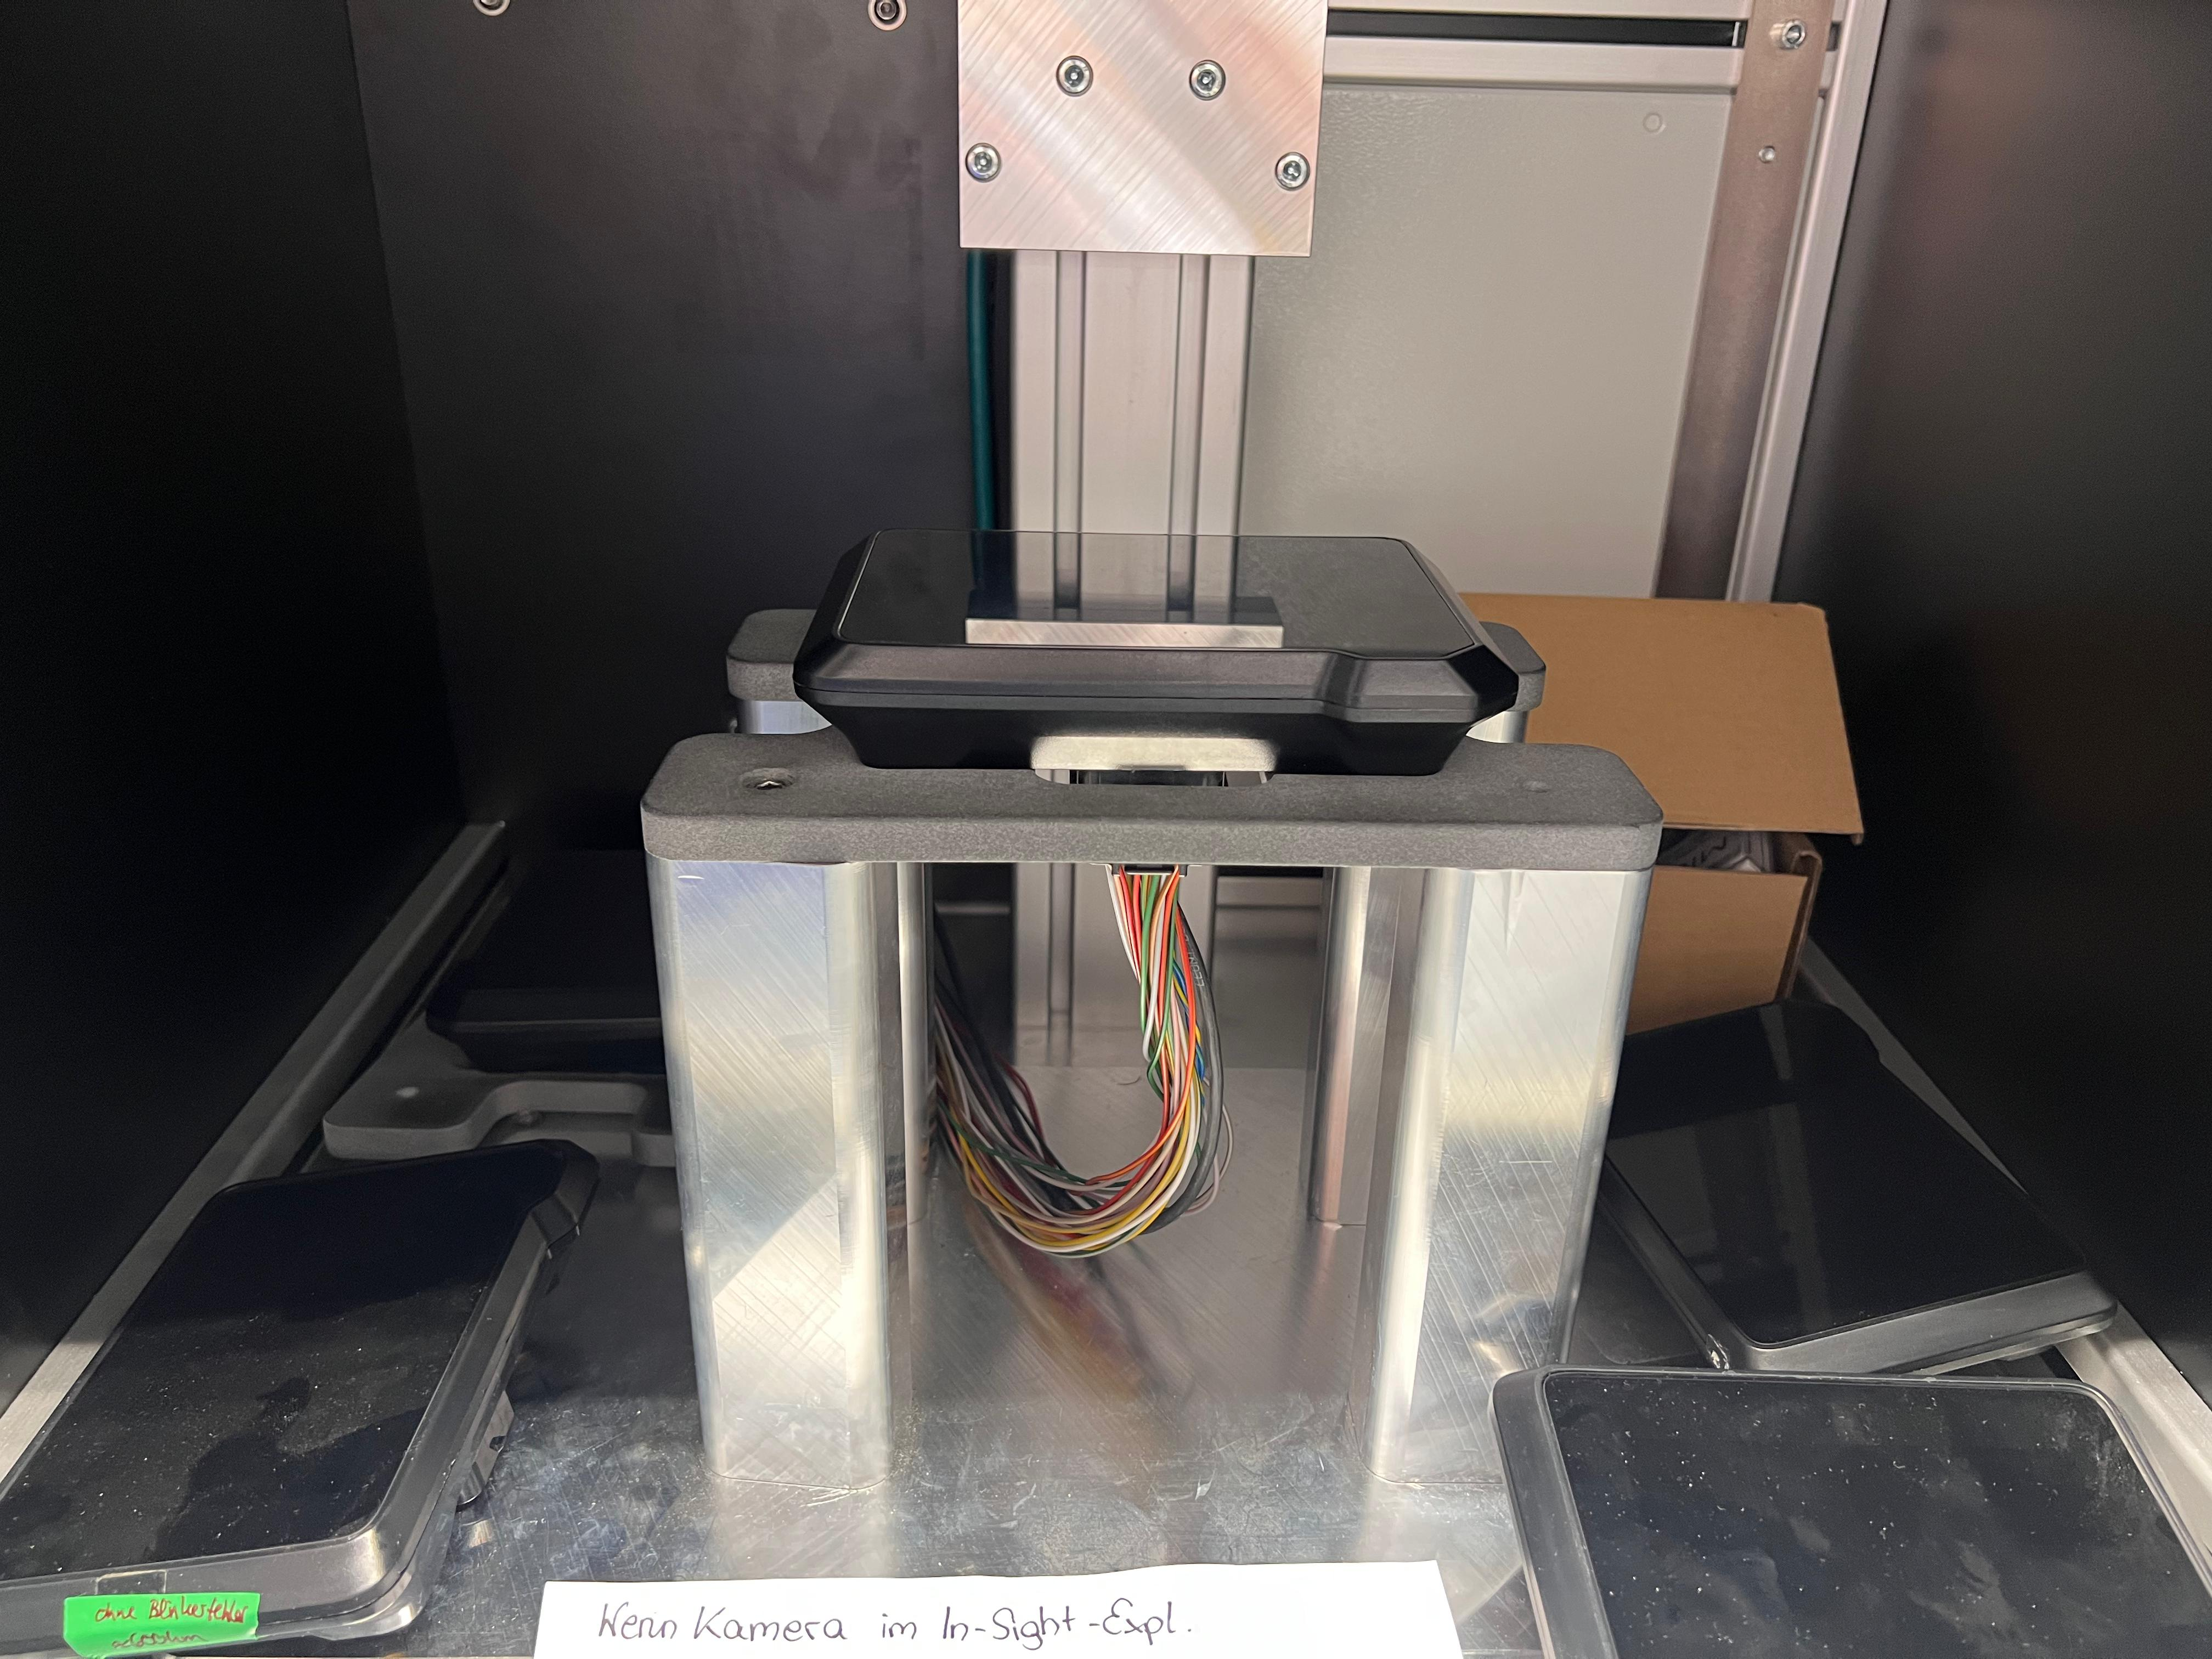
\includegraphics[width=0.6\textwidth]{Figures/db_mounting.jpg}
    \caption{\gls{db} mounted inside the light control box.}
    \label{db_Mounting}
\end{figure}



\subsection{Hardware In The Loop System Integration}



\section{Object Detection Model}
.........
\subsection{Dataset Preparation}
.........
\subsection{Model Training}
.........
\subsection{Model Testing}
.........



\section{System Integration}
.........
\subsection{Model Integration}
.........
\subsection{Data Flow And Processing Pipeline}
.........

